% ============================================================
% AI Workflows and Publishing in Finance
% HKUST PhD Short Course — April 23, 2026
% J. Anthony Cookson
%
% Compile with:  pdflatex slides.tex  (twice for ToC/progress bar)
% Requires: metropolis theme (tlmgr install beamertheme-metropolis)
% ============================================================

\documentclass[aspectratio=169, 10pt]{beamer}

\usetheme[progressbar=frametitle, sectionpage=progressbar,
          numbering=fraction, block=fill]{metropolis}

\usepackage{graphicx}
\usepackage{booktabs}
\usepackage{xcolor}
\usepackage{tikz}
\usepackage{tcolorbox}
\tcbuselibrary{skins, breakable}
\usepackage{fontawesome5}   % icons — remove if not installed
\usepackage{hyperref}
\usepackage{microtype}
\usepackage{setspace}

\graphicspath{{figures/}}

% ── Colour palette ─────────────────────────────────────────
\definecolor{NavyBlue}{HTML}{002855}
\definecolor{SteelBlue}{HTML}{2E6DA4}
\definecolor{LightSteel}{HTML}{D6E4F0}
\definecolor{Coral}{HTML}{C0392B}
\definecolor{PromptBg}{HTML}{FEF9E7}
\definecolor{PromptBorder}{HTML}{F39C12}
\definecolor{FindingBg}{HTML}{EAF4FB}
\definecolor{FindingBorder}{HTML}{2E6DA4}

% ── Theme overrides ────────────────────────────────────────
\setbeamercolor{normal text}{fg=black!85, bg=white}
\setbeamercolor{frametitle}{bg=NavyBlue, fg=white}
\setbeamercolor{progress bar}{fg=SteelBlue, bg=NavyBlue!30}
\setbeamercolor{alerted text}{fg=NavyBlue}
\setbeamercolor{section in toc}{fg=NavyBlue}
\setbeamercolor{block title}{bg=NavyBlue!10, fg=NavyBlue}
\setbeamercolor{block body}{bg=NavyBlue!5, fg=black!85}
\setbeamercolor{block title alerted}{bg=Coral!15, fg=Coral!80!black}
\setbeamercolor{block body alerted}{bg=Coral!5, fg=black!85}
\setbeamercolor{block title example}{bg=SteelBlue!15, fg=SteelBlue!80!black}
\setbeamercolor{block body example}{bg=SteelBlue!5, fg=black!85}

% ── Custom environments ────────────────────────────────────
\newtcolorbox{promptbox}[1][]{
  colback=PromptBg, colframe=PromptBorder,
  boxrule=0.6pt, arc=3pt,
  left=4pt, right=4pt, top=3pt, bottom=3pt,
  fontupper=\small\itshape, #1
}

\newtcolorbox{findingbox}[1][]{
  colback=FindingBg, colframe=FindingBorder,
  boxrule=0.6pt, arc=3pt,
  left=4pt, right=4pt, top=3pt, bottom=3pt,
  fontupper=\small, #1
}

% ── Discussion prompt command ──────────────────────────────
\newcommand{\discussprompt}[1]{%
  \begin{alertblock}{\faComments\quad Discussion}
    \textit{#1}
  \end{alertblock}
}

% ── Title metadata ─────────────────────────────────────────
\title{AI Workflows and Publishing in Finance}
\subtitle{HKUST PhD Short Course}
\author{J.\ Anthony Cookson}
\institute{Penn State Smeal College of Business}
\date{April 23, 2026}


% ============================================================
\begin{document}
% ============================================================

% ── Title ───────────────────────────────────────────────────
{%
\setbeamercolor{background canvas}{bg=NavyBlue}
\setbeamercolor{normal text}{fg=white}
\begin{frame}[plain]
  \vspace{1.5em}
  {\color{white}\Large\bfseries AI Workflows and Publishing in Finance}\\[0.5em]
  {\color{white!70}\large HKUST PhD Short Course}\\[1.5em]
  {\color{white!90} J.\ Anthony Cookson}\\
  {\color{white!70}\small University of Colorado Boulder $\rightarrow$ Penn State Smeal College of Business}\\[0.3em]
  {\color{white!70}\small April 23, 2026}
  \vfill
  {\color{white!50}\footnotesize
    Wiki reference: \href{https://velikov-mihail.github.io/ai-econ-wiki/}{velikov-mihail.github.io/ai-econ-wiki}
    \hfill 3 hours $\cdot$ structured discussion with live demos}
\end{frame}
}

% ── Course goals ────────────────────────────────────────────
\begin{frame}{By the end of this session\ldots}
  \begin{enumerate}
    \setlength{\itemsep}{0.7em}
    \item Set up a \textbf{functional AI workflow} for empirical research ---
          persistent assistant, not a chatbot
    \item Use AI to \textbf{compress the gap} between a dataset and a result
    \item Understand LLMs as \textbf{measurement tools}, not just productivity aids
    \item Reason clearly about how AI is \textbf{changing publishing} and
          what that means for careers starting now
  \end{enumerate}
\end{frame}

% ── Session map ─────────────────────────────────────────────
\begin{frame}{Three blocks, 3 hours}
  \begin{columns}[T]
    \begin{column}{0.23\textwidth}
      \begin{block}{Block 1 \hfill 50 min}
        \textbf{From Skeptic to Power User}\\[0.3em]
        \small Motivation $\cdot$ Blattman framework $\cdot$
        Jagged frontier $\cdot$ Setup
      \end{block}
    \end{column}
    \begin{column}{0.23\textwidth}
      \begin{block}{Block 2 \hfill 70 min}
        \textbf{Empty Folder to Research Result}\\[0.3em]
        \small "Live" demo $\cdot$ Replication packages $\cdot$
        Stress-testing $\cdot$ Literature
      \end{block}
    \end{column}
    \begin{column}{0.23\textwidth}
      \begin{block}{Block 3 \hfill 25 min}
        \textbf{LLMs as Measurement Tools}\\[0.3em]
        \small Market's Mirror as a research application
      \end{block}
    \end{column}
    \begin{column}{0.23\textwidth}
      \begin{block}{Coda \hfill 35 min}
        \textbf{AI and Publishing}\\[0.3em]
        \small Editorial view $\cdot$ Structural changes $\cdot$
        Career implications
      \end{block}
    \end{column}
  \end{columns}
  \vfill
  \begin{center}
    \small\color{black!60}
   
  \end{center}
\end{frame}


% ============================================================
\section{Block 1: From Skeptic to Power User}
% ============================================================

% ── 1.1 Motivation ──────────────────────────────────────────
\begin{frame}{What changed, and why now?}
  The shift is \textbf{not} that AI got better at writing.\\[0.6em]

  It's that AI can now \alert{act} --- read files, run code, manage memory,
  call external services --- inside a project folder that persists across sessions.

  \vspace{0.8em}
  \begin{columns}[T]
    \begin{column}{0.47\textwidth}
      \begin{block}{Vivid example 1}
        A finance paper written in four days\\
        (\textit{``vibe research''})\\[0.2em]
        \small Not an endorsement --- a data point about the frontier.
      \end{block}
    \end{column}
    \begin{column}{0.47\textwidth}
      \begin{block}{Vivid example 2}
        Chris Blattman (UChicago) builds a full AI executive assistant ---
        email triage, project dashboards, calendar, expenses ---
        with no prior coding experience.
      \end{block}
    \end{column}
  \end{columns}
\end{frame}

\begin{frame}{The right framing}
  \vspace{1em}
  \begin{center}
    {\Large ``Become a \alert{complement} to these tools,\\
    not a substitute.''}
  \end{center}
  \vspace{1em}
  \begin{itemize}
    \item The goal is \textbf{not} to automate your research
    \item The goal is to \textbf{eliminate the friction} between your judgment
          and a result
    \item AI speeds up the mechanics; you supply the questions
  \end{itemize}
\end{frame}

% ── 1.2 Blattman Framework ──────────────────────────────────
\begin{frame}{The Blattman Framework}
  \textbf{Site:} \href{https://claudeblattman.com}{claudeblattman.com}
  --- Blattman documented his entire workflow publicly as it evolved.

  \vspace{0.7em}
  \begin{center}
  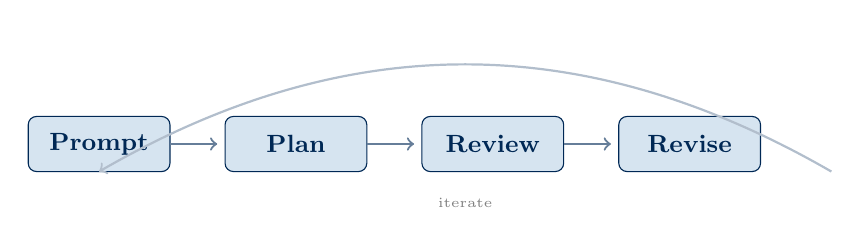
\begin{tikzpicture}[node distance=2.2cm, every node/.style={font=\small}]
    \foreach \label/\x in {Prompt/0, Plan/2.5, Review/5, Revise/7.5} {
      \node[draw=NavyBlue, rounded corners=3pt, fill=LightSteel,
            minimum width=1.8cm, minimum height=0.7cm,
            text=NavyBlue, font=\small\bfseries] at (\x, 0) {\label};
    }
    \foreach \x in {0.9, 3.4, 5.9} {
      \draw[->, thick, NavyBlue!60] (\x, 0) -- (\x+0.6, 0);
    }
    \draw[->, thick, NavyBlue!30, bend right=30] (9.3, -0.35) to (0, -0.35);
    \node[font=\tiny\color{black!50}] at (4.65, -0.75) {iterate};
  \end{tikzpicture}
  \end{center}
  \vspace{0.5em}

  \begin{columns}[T]
    \begin{column}{0.47\textwidth}
      \textbf{The key insight}\\
      \small Value is not in any single output.
      It's in \textit{persistent context} --- a \texttt{CLAUDE.md} that tells
      the assistant who you are, what your projects are, how you want to work.
    \end{column}
    \begin{column}{0.47\textwidth}
      \textbf{Analogy}\\
      \small Like onboarding a very fast RA who never forgets what you've
      told them --- and works 24 hours a day.
    \end{column}
  \end{columns}
\end{frame}

\begin{frame}{\texttt{CLAUDE.md} --- persistent context}
  \begin{columns}[T]
    \begin{column}{0.47\textwidth}
      \textbf{What goes in it:}
      \begin{itemize}
        \item Who you are (role, domain expertise)
        \item Active research projects + co-authors
        \item How you want to communicate
        \item Data sources and file structure conventions
        \item Recurring workflows as named \textit{skills}
      \end{itemize}
    \end{column}
    \begin{column}{0.47\textwidth}
      \textbf{What Blattman built:}
      \begin{itemize}
        \item \texttt{/checkin} --- daily inbox triage + calendar
        \item \texttt{/expenses} --- reimbursement tracking
        \item \texttt{/editor} --- editorial workload dashboard
      \end{itemize}
      \vspace{0.5em}
      \small\color{black!60}
      \textit{Live demo: \texttt{/checkin} in action.}\\
      The goal: make the setup feel achievable, not magical.
    \end{column}
  \end{columns}
  \vfill
  \discussprompt{What's the most time-consuming non-research task in your week?
  Write it down. What would a \texttt{CLAUDE.md} entry for it look like?}
\end{frame}

% ── 1.3 Jagged Frontier ─────────────────────────────────────
\begin{frame}{The Jagged Frontier}
  AI is not uniformly better or worse than a human --- it's \alert{jagged}.

  \vspace{0.5em}
  \begin{columns}[T]
    \begin{column}{0.3\textwidth}
      \begin{exampleblock}{\faCheckCircle\ Trust}
        \small Boilerplate code\\
        Data cleaning\\
        Literature summaries (from docs you provide)\\
        First drafts of methods sections
      \end{exampleblock}
    \end{column}
    \begin{column}{0.3\textwidth}
      \begin{block}{\faSearch\ Verify}
        \small Any specific number or citation it generates\\
        Empirical claims\\
        Package documentation
      \end{block}
    \end{column}
    \begin{column}{0.3\textwidth}
      \begin{alertblock}{\faTimes\ Don't delegate}
        \small Identification strategy\\
        Economic interpretation\\
        Judgment about what's interesting\\
        Referee reports
      \end{alertblock}
    \end{column}
  \end{columns}

  \vspace{0.5em}
  \begin{findingbox}
    The bottleneck is always human verification.
    AI speeds up drafts but creates new review work.
  \end{findingbox}
\end{frame}

% ── 1.4 Setup ───────────────────────────────────────────────
\begin{frame}{Three things that make AI useful vs.\ a toy}
  \begin{enumerate}
    \setlength{\itemsep}{0.8em}
    \item \textbf{\texttt{CLAUDE.md}} --- persistent context file.
          Who you are, your projects, your preferences, your data sources.
          Without this, every session starts cold.

    \item \textbf{Project folders} --- AI works best inside a structured folder
          with data, code, and notes co-located. Think of it as a shared workspace.

    \item \textbf{Skills / commands} --- reusable workflows that encode recurring
          tasks. Write them once; invoke them with a single prompt.
  \end{enumerate}

  \vfill
  \discussprompt{If you were writing a \texttt{CLAUDE.md} for yourself right now
  --- a one-page brief for an AI assistant --- what would be in it?}
\end{frame}


% ============================================================
\section{Block 2: From Empty Folder to Research Result (Research Scoping)}
% ============================================================

% ── 2.0 PGP workflow ────────────────────────────────────────
\begin{frame}{PGP's core insight}
  \begin{center}
    \textit{``AI dramatically shrinks the gap between\\
    a vague research idea and initial results.''}\\[0.3em]
    {\small Paul Goldsmith-Pinkham, BCF Princeton mini-series, March 2026}
  \end{center}

  \vspace{0.7em}
  \begin{enumerate}
    \setlength{\itemsep}{0.4em}
    \item Start with a \textbf{question} and an empty folder
    \item \textbf{Describe} the data you need and where to get it
    \item Let AI \textbf{plan} the pipeline, then iterate
    \item \textbf{Review} outputs at each step --- your judgment is quality control
  \end{enumerate}

  \vspace{0.5em}
  \begin{findingbox}
    The researcher's job: describe the question clearly and review the output
    critically. The code is never the bottleneck --- the questions are.
  \end{findingbox}
\end{frame}

% ── 2.1 Demo setup ──────────────────────────────────────────
\begin{frame}{The demo dataset}
  \begin{columns}[T]
    \begin{column}{0.55\textwidth}
      \textbf{The Social Signal}\\
      Cookson, Lu, Mullins \& Niessner (2024), \textit{JFE}\\[0.4em]
      \small
      \begin{itemize}
        \item 821,534 firm-day observations
        \item 1,500 firms $\times$ 10 years (2012--2021)
        \item Two variables:
          \begin{itemize}
            \item \texttt{zee\_sent\_pc} --- Sentiment PC1 ($z$-score)
            \item \texttt{zee\_attn\_pc} --- Attention PC1 ($z$-score)
          \end{itemize}
        \item First principal component across StockTwits, Twitter, Seeking Alpha
      \end{itemize}
      \vspace{0.4em}
      Publicly available:\\
      \href{https://data.mendeley.com/datasets/xffyybvw4j/1}{\small data.mendeley.com/datasets/xffyybvw4j/1}
    \end{column}
    \begin{column}{0.40\textwidth}
      \begin{block}{The prompt that started it}
        \footnotesize\itshape
        ``I have a firm-day social signal dataset. Help me understand
        what's in it and produce a time-series figure of average sentiment
        and attention. Then merge with Yahoo Finance returns and test whether
        sentiment predicts next-day abnormal returns.''
      \end{block}
    \end{column}
  \end{columns}
\end{frame}

% ── 2.1 Layer 1: firm level ─────────────────────────────────
\begin{frame}{Layer 1 --- Firm-level basics}
  \textbf{From one prompt:} load data $\to$ describe $\to$ time-series figure
  $\to$ return predictability

  \vspace{0.5em}
  \begin{columns}[T]
    \begin{column}{0.50\textwidth}
      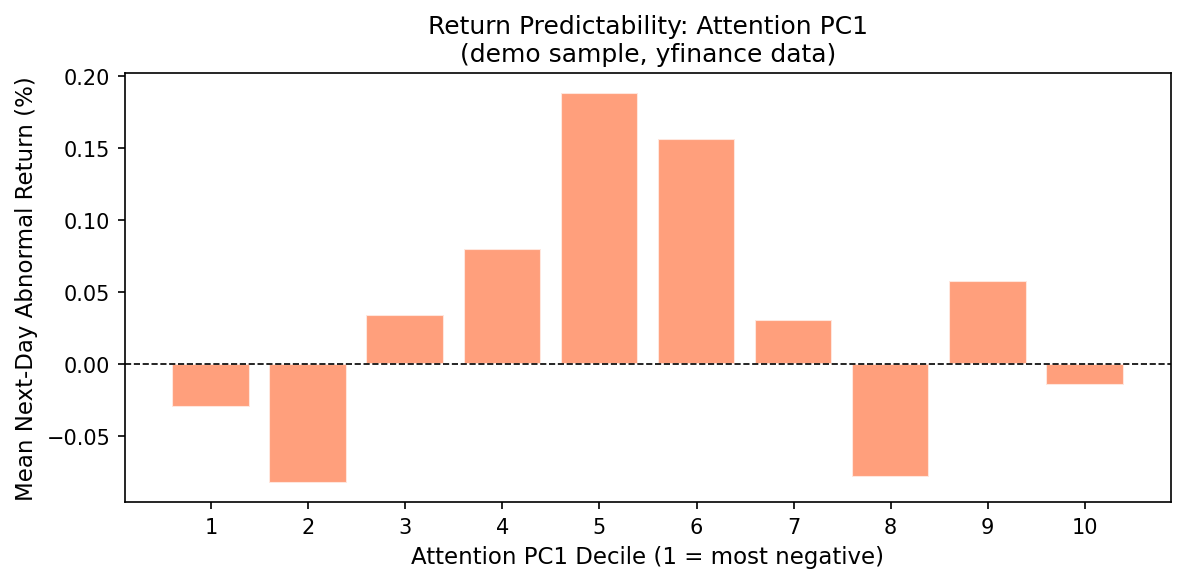
\includegraphics[width=\textwidth]{fig_attn_return_pred.png}
    \end{column}
    \begin{column}{0.46\textwidth}
      \vspace{0.3em}
      \textbf{What this figure shows}\\[0.3em]
      \small
      Return predictability by \textit{attention} decile.
      Decile 1 = least attention; Decile 10 = most.\\[0.5em]

      Higher attention $\to$ \textit{lower} next-day abnormal return.\\[0.5em]

      This is the classic overattention / contrarian pattern:
      when investors pile on, prices overshoot.\\[0.5em]

      Sentiment shows the opposite sign (positive predictability).\\[0.5em]

      \textbf{Signs match Table 6 of the paper.}
    \end{column}
  \end{columns}
\end{frame}

% ── 2.1 Layer 2: market level (prompt) ──────────────────────
\begin{frame}{Layer 2 --- Market-level analysis}
  \begin{promptbox}[title={\small\faKeyboard\ Prompt 2}]
    ``Can you do a demo of how you would produce an aggregate index and
    explore its market-level predictive properties for trading, volatility,
    and returns? Also consider the reverse relation --- how do recent trading,
    vol and returns predict this aggregate index? Does this have anything to
    do with market news events like FOMC dates?''
  \end{promptbox}

  \vspace{0.5em}
  \textbf{What this produced:}
  \begin{itemize}
    \setlength{\itemsep}{0.2em}
    \small
    \item Equal-weighted daily market sentiment \& attention index
    \item Forward regressions: signal $\to$ next-day returns, VIX, volume
    \item Reverse regressions: market outcomes $\to$ signal (Newey-West HAC)
    \item FOMC event study (±15-day window, cumulative return)
    \item Leads-and-lags plot: high vs.\ low signal days
  \end{itemize}
\end{frame}

% ── 2.1 Layer 2: timeseries figure ──────────────────────────
\begin{frame}{The market signal, 2012--2021}
  \begin{center}
    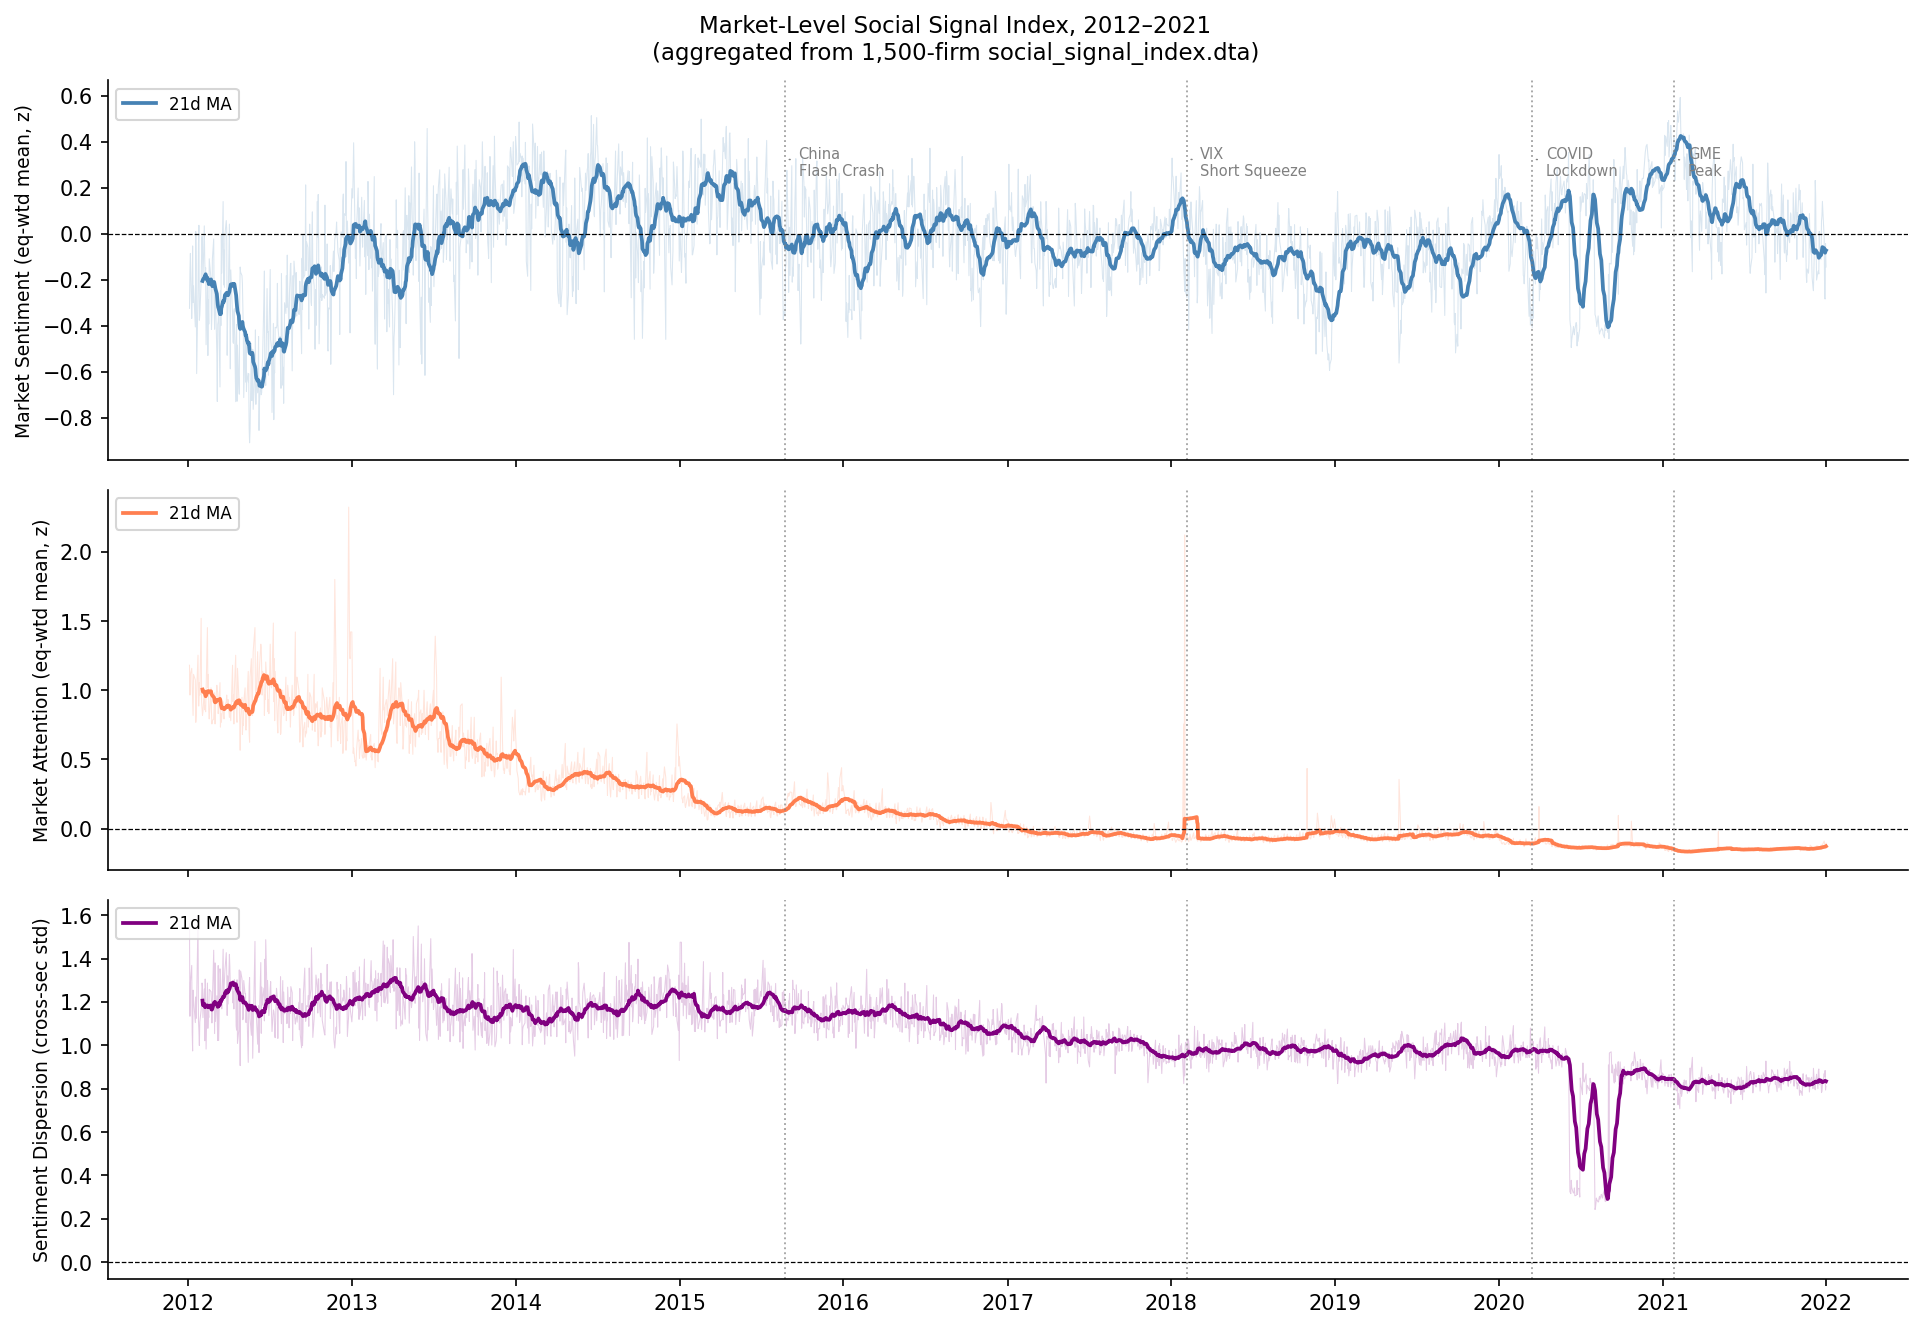
\includegraphics[width=0.92\textwidth]{fig_market_timeseries.png}
  \end{center}
  \vspace{-0.3em}
  {\small\color{black!60}
  Daily equal-weighted cross-sectional mean. Gray dotted lines mark
  China crash (2015), VIX squeeze (2018), COVID lockdown (2020), GME peak (2021).}
\end{frame}

% ── 2.1 Layer 2: leads and lags figure ──────────────────────
\begin{frame}{Leads-and-lags: what happens around high-signal days?}
  \begin{center}
    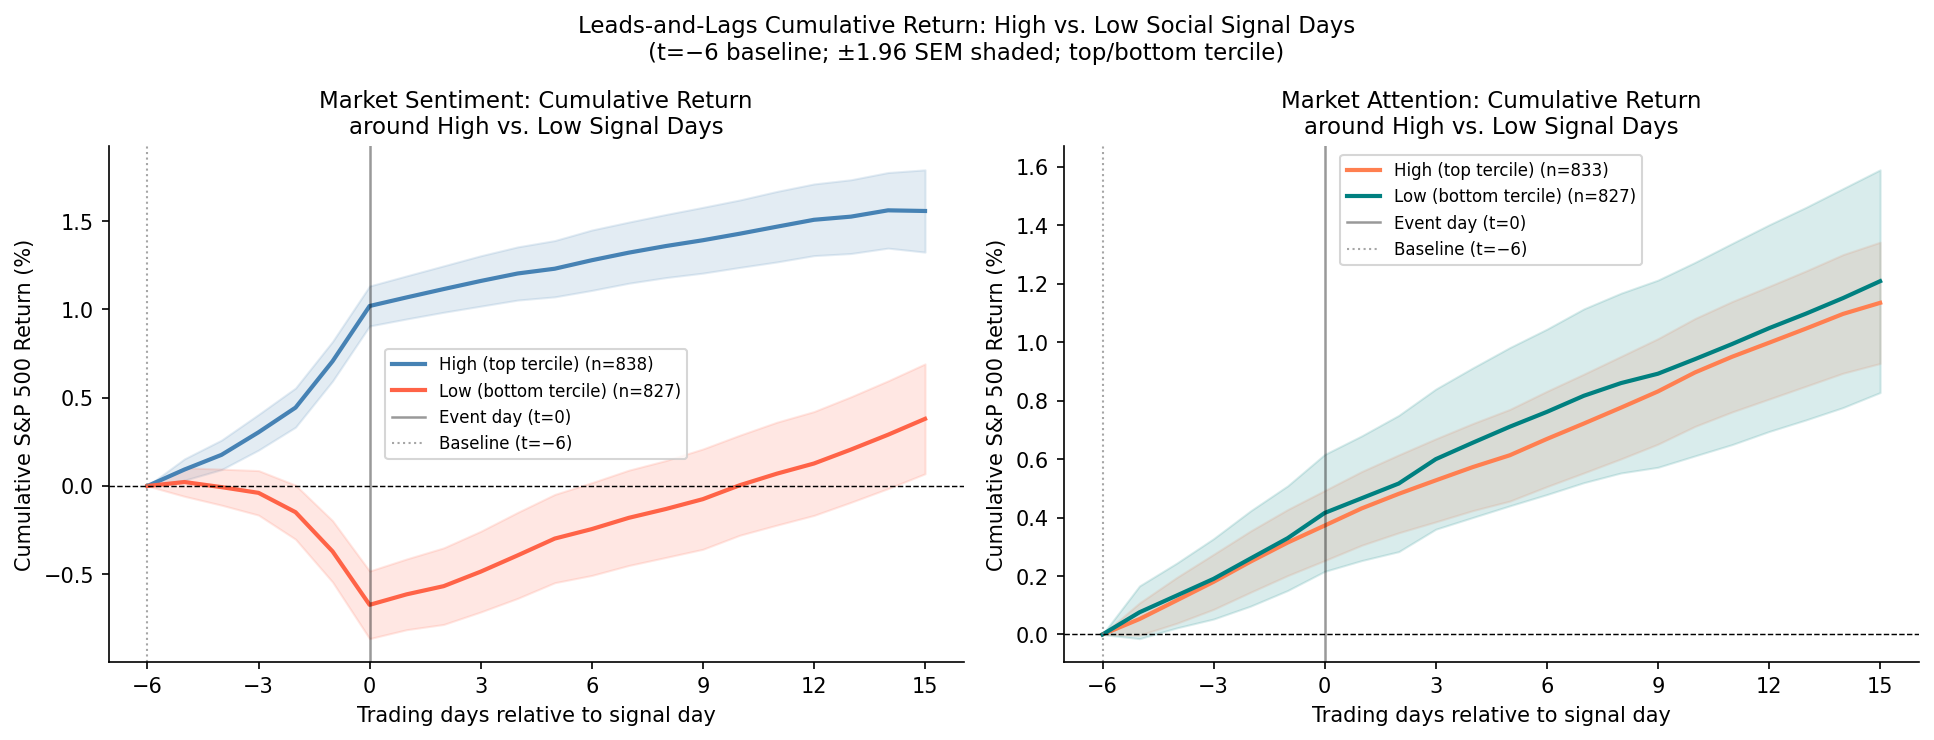
\includegraphics[width=0.92\textwidth]{fig_leads_lags.png}
  \end{center}
  \vspace{-0.3em}
  {\small\color{black!60}
  Event = day in top (blue) or bottom (red) tercile of signal.
  Cumulative S\&P 500 return indexed to 0 at $t{=}-6$; shading = $\pm1.96$ SEM.}
\end{frame}

% ── 2.1 Layer 3: cap-weighted ────────────────────────────────
\begin{frame}{Layer 3 --- Cap-weighted robustness}
  \begin{promptbox}[title={\small\faKeyboard\ Prompt 3}]
    ``Can you aggregate in a market value way and redo the analysis?''
  \end{promptbox}

  \vspace{0.5em}
  \begin{columns}[T]
    \begin{column}{0.50\textwidth}
      \textbf{Three indices compared:}\\[0.2em]
      \small
      \begin{tabular}{lll}
        \toprule
        Index & Coverage & Weight\\
        \midrule
        EW-1500 & All 1,500 firms & Equal\\
        EW-8    & 8 large caps & Equal\\
        CW-8    & 8 large caps & Market cap\\
        \bottomrule
      \end{tabular}
    \end{column}
    \begin{column}{0.46\textwidth}
      \textbf{Key finding:}\\[0.3em]
      \small
      EW-1500 and CW-8 sentiment correlation $r = 0.39$ --- large caps
      diverge meaningfully from breadth-weighted sentiment.\\[0.4em]
      Cap-weighting sharpens predictability
      ($\beta = -0.0007$, $t = -2.13^*$).\\[0.4em]
      Interpretation: \textit{what the mega-caps feel} is a different signal
      from \textit{what the full market feels}.
    \end{column}
  \end{columns}
\end{frame}

% ── 2.1 Demo lesson ─────────────────────────────────────────
\begin{frame}{What the demo illustrates}
  \begin{center}
  \begin{tabular}{p{0.42\textwidth} p{0.42\textwidth}}
    \toprule
    \textbf{Researcher supplied} & \textbf{Claude Code supplied}\\
    \midrule
    Economic question & All Python code\\
    Cap-weighting as a robustness check & Market cap from Yahoo Finance\\
    FOMC event study as the right design & 81 FOMC dates, event panel\\
    ``Leads and lags, not just coefficients'' & Rewrote figure immediately\\
    Benchmark date ($t{=}{-}6$) and window ($t{+}15$) & Cumulative indexing\\
    Whether results make economic sense & All figures and tables\\
    \bottomrule
  \end{tabular}
  \end{center}
  \vspace{0.3em}
  \begin{findingbox}
    Four prompts. $\sim$15 minutes of real session time.
    The code was never the bottleneck. The questions were.
  \end{findingbox}
\end{frame}

% ── 2.2 Structured databases ─────────────────────────────────
\begin{frame}{Larger pipelines: structure matters more}
  When data gets large or messy:
  \begin{itemize}
    \item Convert flat files to Parquet/DuckDB for fast querying \hfill{\small\color{black!50}PGP Episode 4}
    \item Extract structured data from unstructured sources (EDGAR 10-K) \hfill{\small\color{black!50}PGP Episode 3}
    \item \textbf{Planning mode}: ask AI to plan the full pipeline \textit{before} writing any code
    \item \textbf{Sub-agents}: break a complex task into parallel components
  \end{itemize}

  \vspace{0.4em}
  \begin{block}{PGP Episode 4 example}
    \small Mortgage market panel from HMDA data --- county lender
    concentration, fintech/non-bank growth. The kind of data assembly task
    that used to take a RA a month.
  \end{block}

  \discussprompt{Describe a data assembly task in your current project you've
  been putting off because it's tedious. How would you describe it to an AI
  in plain English?}
\end{frame}

% ── 2.2 AI-augmented replication ─────────────────────────────
\begin{frame}{AI-augmented replication packages}
  The same capability that lets you \textit{build} a new pipeline also lets
  you \textit{navigate} an existing one --- with no prior knowledge of the
  codebase.

  \vspace{0.5em}
  \begin{block}{Dickerson, Julliard \& Mueller --- \textit{JFE}}
    \small
    \href{https://github.com/Alexander-M-Dickerson/co-pricing-factor-zoo}{github.com/Alexander-M-Dickerson/co-pricing-factor-zoo}\\[0.3em]
    Replication package ships with a \texttt{.claude/} directory and custom skills:
    \begin{itemize}
      \item \texttt{/onboard} --- validates R, packages, data; auto-fixes gaps
      \item \texttt{/replicate-paper} --- full pipeline with error recovery
      \item \texttt{/explain-paper} --- explains any table or figure on demand
    \end{itemize}
    \vspace{0.2em}
    User prompt: \textit{``Replicate the main text. If packages are missing,
    bootstrap them automatically first.''}
  \end{block}

  \vspace{0.2em}
  \begin{findingbox}
    No prior knowledge of the codebase required.
    This is a new standard for what a replication package can be.
  \end{findingbox}
\end{frame}

% ── 2.3 Stress-testing ──────────────────────────────────────
\begin{frame}{AI as pre-mortem tool}
  Use AI to find the fatal flaw \textit{before} referees do:

  \vspace{0.5em}
  \begin{itemize}
    \setlength{\itemsep}{0.5em}
    \item Describe your identification strategy in a paragraph;
          ask AI to find the holes
    \item \textit{``What would a skeptical referee say about this?''}
    \item \textit{``What's the most obvious alternative explanation?''}
    \item Multiple AI agents auditing your DiD code for specification errors
  \end{itemize}

  \vspace{0.5em}
  \begin{alertblock}{Calibration note}
    AI will also find problems that aren't real.
    You need domain knowledge to filter.
    Use it to generate the list; use your judgment to prioritize.
  \end{alertblock}

  \discussprompt{Describe your current identification strategy in two sentences.
  What's the hardest question you'd get at a seminar?}
\end{frame}

% ── 2.4 Literature and feedback ─────────────────────────────
\begin{frame}{Literature, feedback, iteration}
  \begin{columns}[T]
    \begin{column}{0.47\textwidth}
      \begin{block}{NotebookLM}
        \small Document-grounded AI --- you feed it papers, it reasons over
        them. Much safer than asking AI to recall literature from memory.
        No hallucination risk on documents you provide.
      \end{block}
      \vspace{0.4em}
      \begin{block}{AI referee reports}
        \small Useful as first-pass signal, not a substitute for judgment.
        Good at: missing robustness checks, unclear writing, obvious
        alternative hypotheses.
      \end{block}
    \end{column}
    \begin{column}{0.47\textwidth}
      \begin{block}{Feedback machines}
        \small The iterative loop: draft $\to$ AI critique $\to$ revise
        $\to$ repeat.\\[0.3em]
        Key principle: use AI to \textbf{find weaknesses}, not to
        \textbf{write your paper}.\\[0.3em]
        See also: Refine.ink
      \end{block}
    \end{column}
  \end{columns}
\end{frame}


% ============================================================
\section{Block 3: LLMs as Measurement Tools}
% ============================================================

% ── 3.1 LLMs as instruments ─────────────────────────────────
\begin{frame}{Beyond the assistant: LLMs as research instruments}
  \begin{center}
    {\large LLMs are not just productivity tools.}\\[0.4em]
    {\large They are instruments for \alert{measuring constructs} ---}\\[0.2em]
    {\large beliefs, sentiment, preferences, reasoning ---}\\[0.2em]
    {\large that we couldn't measure at scale before.}
  \end{center}
\end{frame}

% ── 3.1 Market's Mirror ─────────────────────────────────────
\begin{frame}{Case study: The Market's Mirror}
  \textbf{Cookson, Bhagwat, Dim \& Niessner} (working paper)\\[0.5em]

  \textbf{Question:} How do demographics drive investor disagreement?
  Does demographic disagreement predict trading?

  \vspace{0.5em}
  \begin{columns}[T]
    \begin{column}{0.50\textwidth}
      \textbf{The approach:}
      \begin{itemize}
        \small
        \item Imbue Llama 3.1 8B with \textbf{216 investor personas}\\
              (72 demographic combos $\times$ 3 political orientations,\\
              weighted by FINRA survey data)
        \item Ask all 216 personas for buy/hold/sell on\\
              \textbf{5.5 million} S\&P 500 news headlines (2010--2025)
        \item Weighted SD of sentiment $=$ LLM disagreement measure
      \end{itemize}
    \end{column}
    \begin{column}{0.46\textwidth}
      \textbf{Why this is methodologically novel:}
      \begin{itemize}
        \small
        \item A \textit{survey that could not be done with humans}\\
              (1.188 billion items)
        \item Allows revision: update the paper, re-query the same way
        \item Fixed training window $\to$ post-training validation (2024--25)
      \end{itemize}
    \end{column}
  \end{columns}
\end{frame}

\begin{frame}{What the Market's Mirror finds}
  \begin{columns}[T]
    \begin{column}{0.48\textwidth}
      \textbf{Key findings:}
      \begin{itemize}
        \small
        \item Income and politics drive disagreement most
        \item Social/soft news generates more disagreement than hard
              financial news
        \item LLM disagreement validates against human survey data
              (Iliewa et al.\ 2025; Toubia et al.\ 2025 digital twins)
        \item Disagreement predicts abnormal trading volume,
              especially retail trading
      \end{itemize}
    \end{column}
    \begin{column}{0.48\textwidth}
      \begin{findingbox}
        \textbf{The broader point:}\\[0.3em]
        \small This opens an entire new research agenda.
        Any latent construct --- beliefs, preferences, reasoning styles ---
        that you can elicit from a persona can now be measured at scale.\\[0.3em]
        What questions become answerable that weren't before?
      \end{findingbox}
    \end{column}
  \end{columns}

  \vspace{0.3em}
  \discussprompt{What latent construct in your research area would you want to
  measure at scale if you could run 1 billion surveys?
  What would the right instrument look like?}
\end{frame}

% ── Transition ──────────────────────────────────────────────
\begin{frame}{The common thread}
  Three demonstrations, three layers of capability:
  \vspace{0.4em}
  \begin{enumerate}
    \setlength{\itemsep}{0.5em}
    \item \textbf{AI accelerates the workflow} --- from \texttt{CLAUDE.md}
          to \texttt{/checkin}, friction between judgment and result collapses
    \item \textbf{AI builds and navigates research pipelines} --- 821k
          firm-days to market-level analysis in four prompts, $\sim$15 minutes
    \item \textbf{AI enables measurement at impossible scale} --- 216 personas,
          5.5 million headlines, 1.188 billion elicitations
  \end{enumerate}
  \vspace{0.6em}
  \begin{findingbox}
    In every case, research got \textbf{faster} \textit{and} \textbf{better}.\\[0.2em]
    \small Not faster \textit{or} better. Both at once.
    That is worth pausing on before we ask what it means for publishing.
  \end{findingbox}
\end{frame}


% ============================================================
\section{AI and the Future of Publishing}
% ============================================================

% ── Editorial perspective ────────────────────────────────────
\begin{frame}{From the editor's desk}
  \textit{A view from $\sim$10 new manuscripts per month across
  Management Science and RCFS\ldots}

  \vspace{0.5em}
  \begin{columns}[T]
    \begin{column}{0.47\textwidth}
      \begin{exampleblock}{What's getting better}
        \small Writing is better, but this is mostly a Chatbot effect that has shown up already.
        I have seen more obvious AI-written reports on my own work than among my referees.
      \end{exampleblock}
    \end{column}
    \begin{column}{0.47\textwidth}
      \begin{alertblock}{What's getting harder}
        \small More submissions. More polished-looking work.
       
       Interesting tension: I evaluate more on the quality of the idea. This can be easier to sort out once everything is written passably. 
      \end{alertblock}
    \end{column}
  \end{columns}

  \vspace{0.5em}
  \begin{findingbox}
    True separation will come from using these tools in support of better ideas.  \\
    Skepticism: AI doesn't (yet?) ideate well.  Will it ever?
  \end{findingbox}
\end{frame}

% ── 3.2 Publishing ──────────────────────────────────────────
\begin{frame}{Research and publishing are decoupling}
  \begin{center}
    {\large ``Research and publishing are now two different things.''}
  \end{center}
  \vspace{0.5em}
  \begin{itemize}
    \setlength{\itemsep}{0.4em}
    \item AI lowers the cost of a \textit{plausible-looking} paper to near zero
    \item On the flip side, \textbf{truth-seekers} are enabled by these tools.
     \item How can we --- as a profession --- combat HARK'ing \& encourage discovery?
  \end{itemize}
  \vspace{0.4em}
  \begin{columns}[T]
    \begin{column}{0.47\textwidth}
      \begin{block}{The supply side}
        \small AI one-shot papers, vibe research, automated policy evaluation
        (Project APE) --- these exist and will improve.
      \end{block}
    \end{column}
    \begin{column}{0.47\textwidth}
      \begin{alertblock}{The quality filter}
        \small Replication and robustness become \textit{easier} to demand.
        Editors will raise the bar.
        The threshold for ``publishable'' rises with the supply of cheap papers.
      \end{alertblock}
    \end{column}
  \end{columns}
\end{frame}

\begin{frame}{Replication packages as a new norm}
  Tie back to Dickerson et al.\ (Block 2):
  if AI can replicate a paper in one command, editors can \textit{require} it.

  \vspace{0.5em}
  \begin{columns}[T]
    \begin{column}{0.47\textwidth}
      \textbf{For accountability:}\\
      \small Your identification strategy and code become legible to anyone
      with Claude Code --- reviewers, competitors, editors.
      Methodological transparency is no longer optional.
    \end{column}
    \begin{column}{0.47\textwidth}
      \textbf{For leverage:}\\
      \small You can build on others' work faster.
      A well-documented, AI-navigable package is a contribution that gets
      cited and used.\\[0.4em]
    \end{column}
  \end{columns}
\end{frame}

\begin{frame}{What this means for your career}
  The premium will shift toward:
  \begin{itemize}
    \setlength{\itemsep}{0.5em}
    \item \textbf{Deep domain knowledge} --- AI can't (yet?) supply the economic
          question (will it?)
    \item \textbf{Identification creativity} --- insightful research (and refereeing) still
          requires human judgment
    \item \textbf{Real-world access} --- proprietary data, field experiments,
          regulatory relationships
    \item \textbf{Measurement novelty} --- like the LLM persona approach ---
          as a source of edge
  \end{itemize}

  \vspace{0.5em}
  \discussprompt{What are you building that AI can't replicate?
  And what part of your current workflow are you doing manually that AI
  could handle tomorrow?}
\end{frame}

% ── 3.3 Open questions ──────────────────────────────────────
\begin{frame}{Genuine uncertainty --- open questions}
  No settled answers on:
  \vspace{0.3em}
  \begin{itemize}
    \setlength{\itemsep}{0.5em}
    \item How fast autonomous research agents arrive and how good they get, especially at ideating
    \item Whether LLM measurement tools will be accepted as identification
          or dismissed as fancy text mining
    \item Where the satisfaction in research comes from once discovery is cheap (Scott Cunningham perspective).  Is discovery cheap?
  \end{itemize}
\end{frame}

% ── Closing ─────────────────────────────────────────────────
\begin{frame}{To close}
  \discussprompt{What is one thing you'll do differently in your research
  workflow this week?\\[0.4em]
  And what is the question about AI and research that you most want answered?}

  \vfill
  \begin{center}
    \small\color{black!60}
    Course materials 
    Wiki: \href{https://velikov-mihail.github.io/ai-econ-wiki/}{velikov-mihail.github.io/ai-econ-wiki}
    \quad$\cdot$\quad
    \href{https://claudeblattman.com}{claudeblattman.com}
    \quad$\cdot$\quad
    \href{https://bcf.princeton.edu/events/paul-goldsmith-pinkham-mini-series-on-claude-code-for-applied-economists/}{PGP mini-series (BCF Princeton)}
  \end{center}
\end{frame}


% ── Backup / Appendix ───────────────────────────────────────
\appendix

\begin{frame}{Selected readings}
  \textbf{Conceptual}
  \begin{itemize}
    \small
    \item ``The Shape of AI: Jaggedness, Bottlenecks and Salients'' (Velikov wiki)
    \item ``Research and Publishing Are Now Two Different Things'' (Velikov wiki)
    \item ``The Bitter Lesson'' --- Rich Sutton
  \end{itemize}
  \vspace{0.4em}
  \textbf{Practical}
  \begin{itemize}
    \small
    \item PGP Episode 1: \href{https://paulgp.substack.com/p/getting-started-with-claude-code}{paulgp.substack.com}
    \item PGP Episode 2: \href{https://paulgp.substack.com/p/from-an-empty-folder-to-a-figure}{From an empty folder to a figure}
    \item \href{https://claudeblattman.com}{claudeblattman.com} --- browse the workflows
  \end{itemize}
  \vspace{0.4em}
  \textbf{For the ambitious}
  \begin{itemize}
    \small
    \item Korinek, ``Generative AI for Economic Research: Use Cases and Implications''
    \item ``Feedback Machines: Writing and Editing Research Papers with AI''
    \item Dickerson et al.\ co-pricing replication package (AI-ready example)
  \end{itemize}
\end{frame}

\begin{frame}{The demo package}
  All code, figures, and prompt logs are in the course repository:
  \vspace{0.5em}
  \begin{block}{Market-Level Analysis demo}
    \small
    \texttt{demos/Market-Level Analysis/}\\[0.2em]
    \texttt{\ \ market\_analysis.py} --- equal-weighted baseline\\
    \texttt{\ \ market\_analysis\_capweighted.py} --- cap-weighted comparison\\
    \texttt{\ \ demo\_guide.md} --- full prompt log + pedagogical notes\\[0.3em]
    Run either script to reproduce all figures from scratch in $\sim$30 seconds.
  \end{block}
  \vspace{0.4em}
  \begin{block}{Social Signal Demo}
    \small
    \texttt{demos/Social Signal Demo/demo\_script.py}\\[0.2em]
    Loads \texttt{social\_signal\_index.dta}, merges with Yahoo Finance,
    produces return predictability figures. No proprietary data needed.
  \end{block}
\end{frame}

\end{document}
